\documentclass[runningheads,envcountsect]{llncs}

\usepackage[margin=2.5cm]{geometry}
% HACK to use titlesec
%% Save the class definition of \subparagraph
\let\llncssubparagraph\subparagraph
%% Provide a definition to \subparagraph to keep titlesec happy
\let\subparagraph\paragraph
%% Load titlesec
\usepackage[compact]{titlesec}
%% Revert \subparagraph to the llncs definition
\let\subparagraph\llncssubparagraph

\usepackage{algorithmic}
\usepackage[utf8]{inputenc}
\usepackage[english]{babel}
\usepackage{amsmath}
\usepackage{amssymb}
\usepackage{mathtools}
\usepackage{enumitem}
\usepackage{float}
\usepackage[colorlinks=true,
            urlcolor=blue,
            linkcolor=black,
            citecolor=blue]{hyperref}
\usepackage{pbox}
\usepackage{framed}
\usepackage{array}
\usepackage{todonotes}
\usepackage{graphicx}

% title resize
\titleformat*{\section}{\fontsize{14}{16}\selectfont\bfseries}
\titleformat*{\subsection}{\fontsize{12}{20}\selectfont\bfseries}

% float environment for schemes
\floatstyle{boxed}
\newfloat{scheme}{ht}{lo}
\floatname{scheme}{Scheme}
\newcommand{\schemeautorefname}{Scheme}

\floatstyle{boxed}
\newfloat{gamehop}{ht}{lo}
\floatname{gamehop}{Game Hop}
\newcommand{\gamehopautorefname}{Game Hop}

% environment for exercises
\spnewtheorem{mpkcexercise}{Exercise}[section]{\bfseries}{\rmfamily}
\spnewtheorem{mpkcproof}{Proof}[section]{\bfseries}{\rmfamily}
\setcounter{secnumdepth}{3}

% some useful sets
\newcommand{\G}{\ensuremath{\mathbb{G}}}
\newcommand{\Z}{\ensuremath{\mathbb{Z}}}
\newcommand{\N}{\ensuremath{\mathbb{N}}}
\newcommand{\M}{\ensuremath{\mathcal{M}}}
\newcommand{\A}{\ensuremath{\mathcal{A}}}
\newcommand{\R}{\ensuremath{\mathcal{R}}}
\newcommand{\B}{\ensuremath{\mathcal{B}}}
\renewcommand{\O}{\ensuremath{\mathcal{O}}}
\newcommand{\V}{\ensuremath{\mathcal{V}}}
\renewcommand{\P}{\ensuremath{\mathcal{P}}}


% Center text in table with custom size
\newcolumntype{C}[1]{>{\centering\arraybackslash}p{#1}}


% x \getsr X to sample x from X uniformly at random
\newcommand{\getsr}
  {{\:{\gets{\hspace*{-9pt}\raisebox{5pt}{$\scriptscriptstyle{R}$}}}\hspace*{3.3pt}}}

\title{{\huge Reinforcement Learning Approach on the Order Scheduling for the RoboCup Logistic league}\\{\LARGE \vspace{4pt} by Khodachenko Ian}}
\titlerunning{RCLL scheduling (revision 1.0)}
\author{}
\institute{}

\begin{document}

\maketitle

\section{Robo Cup Logistic League Motivation}
The Robo Cup Logistics League (RCLL) is designed to represent a common scenario in Industry $4.0$. Here one needs to assemble products based on dynamic custom orders in a real-time environment. This means that the environment is driven by a consistent stream of orders and individual delivery windows, which dictate the steps robots in the environment need to take. The challenge here consists in scheduling the assembly process of orders in a feasible manner, to abide the delivery window of as many orders as possible, to figure out priorities or complexities and to understand which orders can't be completed in time.

\section{Reinforcement Learning approach}
We present a solution based on Reinforcement Learning (RL) to tackle the problem of deciding which assembly step the robots need to process next. Due to the complexity of the problem a Deep Q-Learning (DQL) approach is initially applied, while keeping open options and alternatives described in section \ref{risks}.\\
The goal of Q-learning is for an agent to select actions, which maximize the total reward earned over an episode (=game), by observing the state and reward from the environment (see figure \ref{fig:rl}). So from a state $s$ and action $a$ we want to get the maximum future reward $r$, which we denote as the Q-value $Q(s,a)=r(s,a)+\gamma max_a Q(s',a)$. With hyper parameter $\gamma$ we can scale the future rewards.\\
To shift from Q-learning to DQL we apply a Deep Neural Network (DNN or DQN) to learn the Q-values for each individual action, given a state (see figure \ref{fig:dql}). We can update the DNN via stochastic gradient descent and backpropagation from a squared error loss on the target $Q_\theta(s,a)$. The $\theta$ is the policy we want to optimize. Since in contrast to a normal DNN scenario, here we have to update the target we are learning (like cutting the branch one sits on), we need to set-up two parallel networks like in figure \ref{fig:rl_dm}. From figure \ref{fig:rl_dm} one can see that we work with two networks of identical achitecture and fix the target network weights, while training the prediction network. The weights are copied over to the target network every $C$ iterations and enable us to form a more stable policy $\theta$. As an addition to this we apply experience replay, by storing a number of $(s_t, a_t, r(s_t, a_t), s_{t+1})$ tuples, which we can reuse reducing total data needed.\\
Putting all together we arrive at figure \ref{fig:dql_full}, which roughly translates to
\begin{enumerate}
	\item Giving the current state to the DQN, which returns the Q-values for all possible actions.
	\item Selection a possible action with an $\epsilon$-greedy policy, where we select a random action with probability $1-\epsilon$ or the action with the maximum Q-value $max_a Q(s,a)$.
	\item Proceed to next state taking the selected action and receiving respective reward. Also storing the transition in the replay memory.
	\item Sample random batches of transitions from the replay buffer to compute the loss $L= (r + \gamma max_{a'} Q_{\theta'}(s', a') - Q_\theta(s, a))^2$.
	\item Perform gradient descent minimizing the loss for the prediction network.
	\item Every $C$ iteration copy the weights of the prediction network to the target network.
	\item Repeat all of the above for a number of episodes.
\end{enumerate}

\begin{figure}[h!]
  \centering
  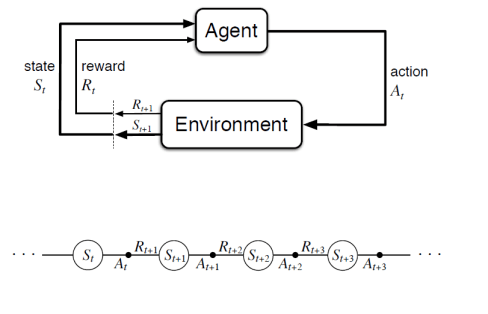
\includegraphics[scale=0.7]{img/rl_base.png}
  \caption{Basic idea of Reinforcement Learning.}
  \label{fig:rl}
\end{figure}

\begin{figure}[h!]
  \centering
  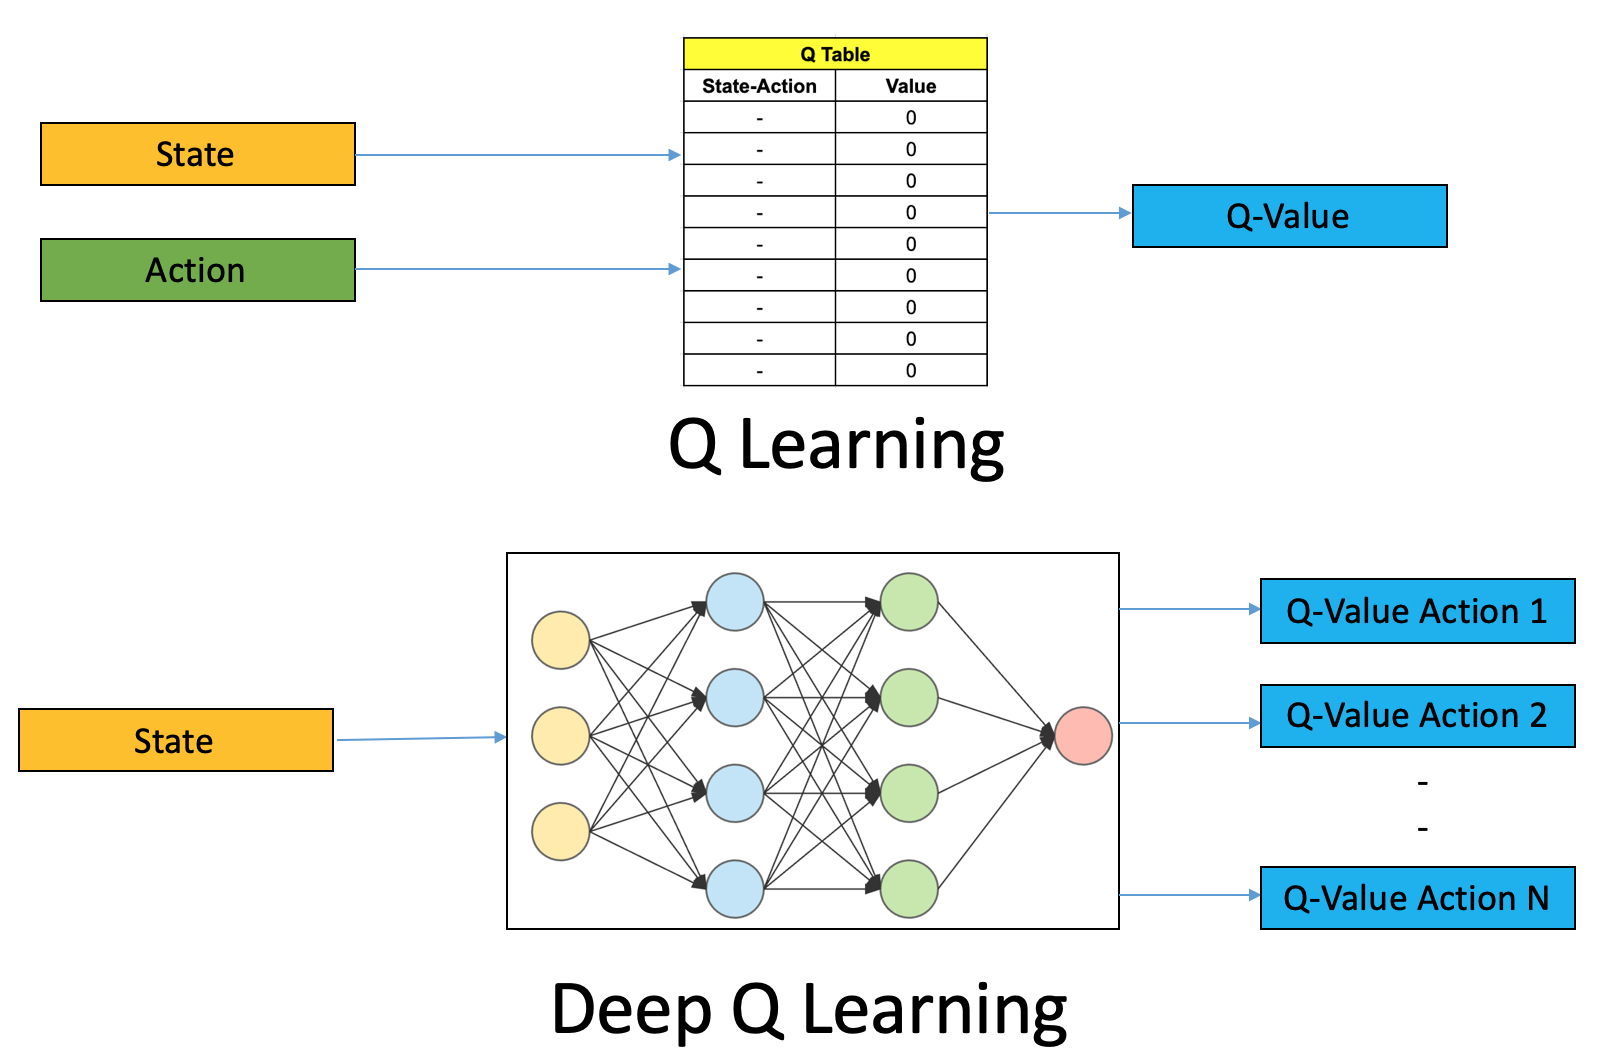
\includegraphics[scale=0.3]{img/dql.png}
  \caption{Comparison of using a Q-table and a neural network.}
  \label{fig:dql}
\end{figure}

\begin{figure}[h!]
  \centering
  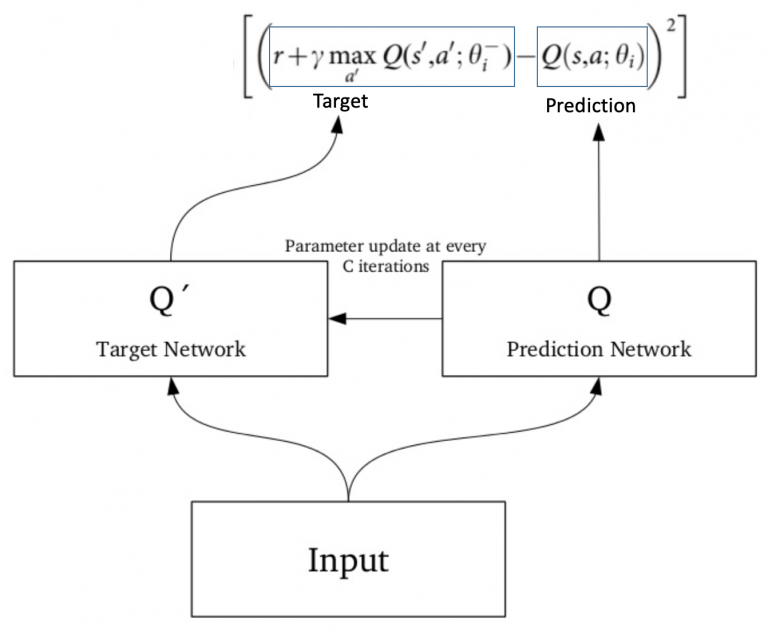
\includegraphics[scale=0.3]{img/rl_double_model.png}
  \caption{Structure for updating the two internal networks in the RL set-up.}
  \label{fig:rl_dm}
\end{figure}

\begin{figure}[h!]
  \centering
  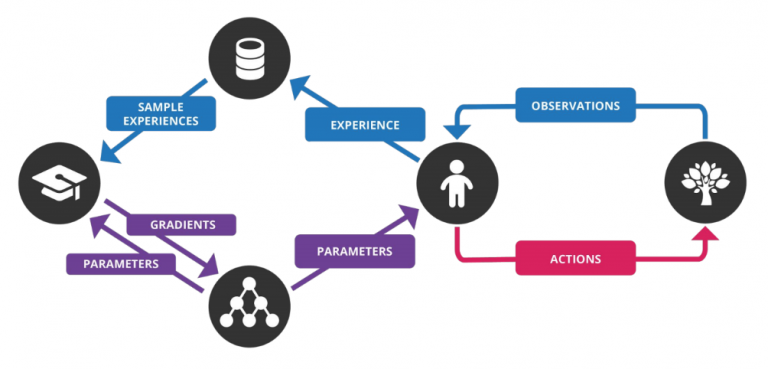
\includegraphics[scale=0.5]{img/dql_full.png}
  \caption{Structure for the full DQL cycle.}
  \label{fig:dql_full}
\end{figure}


\subsection{Environment} \label{env}
In the first steps we apply a more simplified environment, which only provides an order schedule with delivery windows. The initial goal is thus for the system to learn which orders are most feasible to complete or award most rewards.\\
We build the environment so that we can have a precision of seconds, while not specifically modelling each second as a discrete time step. The idea is to merge the discrete time into the actual state as a numerical feature, which is incremented in the expected passed time for a processing step. Initially the elapsed time for the intermediate steps is drawn from Gaussian distributions, which can be later extended with application of the distance matrix and real-world data.\\
Each task $t_k$ will depend on the duration for a sub-step needed to complete order $O=\sum_{i=0}^N t_i$ and will be modelled as $t_k = \mathcal{N}(\mu_k, \sigma_k^2) + \mathcal{U}(a_M,b_M)$. Here the normal distribution $\mathcal{N}$ is given by $\mu_k=d_{ij}$ drawn from a distance matrix representing the distance between machines $M_i$ and $M_j$. The $\sigma_k$ can either be fine-tuned by hand or matched from real recorded robot data. So in other words $\mathcal{N}$ estimates the time a robot will take to move. For the uniform distribution $\mathcal{U}$ we adapt the values given from the rulebook, which represent random uniform processing time at the specific machine $M$.\\
The environment will handle the internal states, which include the playing field distances, product schedule, and robot locations. It will support OpenAI-gym conform functions and more optimizations. The environment can handle communication with the RefBox for the RCLL, to pull out the game field and intermediate points as rewards. The reason for this is to learn the specific official implementation and maximize the rewards based on the official tool, as there may be inconsistencies to the rulebook and the environment needs no updates on rule changes (as those are implemented in the RefBox by the official parties).

\subsection{States} \label{states}
The state space consists of orders, up to 3 products in the pipeline, distance matrix of the machines, availability of machines and current time (the position of the robot should be deductible from last state). While the distance matrix is constant throughout an episode, the other parameters are simulating a dynamic real-time environment.\\
Specifically we can represent an order as a vector of $O=\{\mathcal{B}, \mathcal{R}_1, \mathcal{R}_2, \mathcal{R}_3, \mathcal{C}, n, c, d_{start}, d_{end}  \}$, where
\begin{itemize}
  \item $\mathcal{B}$ represents a set of base types
  \item $\mathcal{R}$ is one of up to 3 ring types
  \item $\mathcal{C}$ is the cap type
  \item $n$ is the requested amount
  \item $c$ indicates whether the order is competitive
  \item $d_{start}$ is the start of the delivery window
  \item $d_{end}$ is the end of the delivery window
\end{itemize}
A intermediate product in the pipeline will look like $\{\mathcal{B}, \mathcal{R}_1, \mathcal{R}_2, \mathcal{R}_3\}$, which corresponds to the physical object one of the 3 robots can transport. We can also omit the cap as we will deliver straight after.\\
The distance matrix is computed at the start of the episode and the machine availability is as the game dictates.\\
While there is still room for changes the current dimensions are ...


\subsection{Actions}
The actions consist of selecting $A=\{\mathcal{B}_P, \mathcal{R}_P, \mathcal{C}_P, d_P\}$, which is a base, ring, cap or discarding the product in pipeline $P$. By discarding we order the option to discontinue the current order and use the pipeline slot for another. In total we have an action space of $A\cdot P$.


\subsection{Rewards}
The initial idea for the rewards is that they should strongly mirror the current rewards assigned by the RefBox, to optimize the points gained in an actual game using the RefBox's rulebook implementation. There are just minor additions to the rewards, like e.g. adding some for acquiring bases to stimulate the learning of the network. This point may see more changes later in the development process, as it is one of the main ways to regulate the learned policy.


\subsection{Risk mitigation} \label{risks}
For DQL to work we make sure the Markov property holds, i.e., that each state only depends on the previous state and the transition from that state to the current one. For this reason we need to make sure that the states provide all the needed information, so the above design is not completely fixed and may be updated later.\\
As such here one will find possible fallback strategies and properties in no particular order:

\begin{itemize}
  \item We avoid using a multi-agent model by focusing on the order schedule and deducting a task sequence based on it. This task sequence can be forwarded from the GRIPS Teamserver to the individual robots and the time they take will be modelled as described in section \ref{env}.
  \item If we need to reduce complexity or in contrast intertwine the actual robot movement deeper into the model, we can apply similar multi-skill and multi-machine approaches as described in \cite{qu2016optimized}.
  \item In the case where the estimation of time consumption for the specific tasks do not represent the real world well enough, we can train an additional neural network in a supervised manner. Here the inputs would be from measured data for given machine distance matrix - to give us more accurate estimations for the expected time consumption at a specific task.
  \item When the communication with the RCLL RefereeBox, becomes problematic the rules can be manually translated into the environment.
  \item Initially we will model by only allowing allowing valid actions (similar to Google Deep Mind), which consist in allowing only process known orders (not guessing future orders), but this can be changed by assigning negative rewards to the guessed order steps.
  \item There is a possibility that the model will possibly disregard the delivery windows as (per official reward structure) the assembly of more difficult products yields much more then the timely delivery.
\end{itemize}


\section{Main development schedule}
First we try to build a network which can assemble a single order by selecting from the actions. Next we want it to recognize and understand the time it will take to process a single order, with a constant distance between machines. To do this we want it to be able to select from a number of orders and try to understand the delivery window.\\
The environment will be extended as needed and the reward and action space will be adjusted as well. This should enable scaling up the difficulty and observe the feasibility of the DQN approach.


\vspace{24pt}

\bibliographystyle{alpha}
\bibliography{description.bib}

\end{document}
